%%%%%%%%%%%%%%%%%%%%%%%%%%%%%% Preamble
\documentclass{article}
\usepackage{amsmath,amssymb,amsthm,fullpage}
\usepackage[a4paper,bindingoffset=0in,left=1in,right=1in,top=1in,
bottom=1in,footskip=0in]{geometry}
\newtheorem*{prop}{Proposition}
%\newcounter{Examplecount}
%\setcounter{Examplecount}{0}
\newenvironment{discussion}{\noindent Discussion.}{}
\setlength{\headheight}{12pt}
\setlength{\headsep}{10pt}
\usepackage{fancyhdr}
\pagestyle{fancy}
\fancyhf{}
\lhead{CS144 HW 1}
\rhead{Matt Lim}
\pagenumbering{gobble}
\usepackage{graphicx}
\usepackage{bbm}
\graphicspath{ {.} }
\begin{document}

\noindent \textit{Collaborated with Kshitij Grover and Siddharth Murching}

%%%%%%%%%%%%%%%%%%%%%%%%%%%%%% Problem 1
\section*{Problem 1}
\subsection*{(a)}
\subsubsection*{(i)}
We know the following inequality involving random variables is true (it can
be easily checked for the two indicator value values):

\[ t \mathbbm{1}_{X \geq t} \leq X \]

Then, since expectation satisfies monotonicity and linearity, we have that

\[ t E[\mathbbm{1}_{X \geq t}] \leq E[X] \]

Finally, given that $E[\mathbbm{1}_A] = P(A)$, we have that

\[ P(X \geq t) \leq \frac{E[X]}{t} \]

\subsubsection*{(ii)}
We know the following inequality involving random variables is true (it can
be easily checked for the two indicator value values):

\[ t \mathbbm{1}_{|X - E[X]| \geq t} \leq |X - E[X]| \]
\[ t^2 \mathbbm{1}_{|X - E[X]| \geq t} \leq (X - E[X])^2 \]

Then, since expectation satisfies monotonicity and linearity, we have that

\[ t^2 E[\mathbbm{1}_{X - E[X] \geq t}] \leq E[(X - E[X])^2] \]

Next, given that $E[\mathbbm{1}_A] = P(A)$, we have that

\[ P(X - E[X] \geq t) \leq \frac{E[(X - E[X])^2]}{t^2} \]

Finally, since we can write $Var(X) = E[(X - E[X])^2] = \sigma_X^2$, we have that

\[ P(X - E[X] \geq t) \leq \frac{\sigma_X^2}{t^2} \]

\subsubsection*{(iii)}
We will first show that $E[\frac{S_n}{n}] = E[X]$. 

\[ E[\frac{S_n}{n}] = E[\frac{\sum_{i = 1}^n X_i}{n}] \]
By linearity of expectation, and since $n$ is a constant, we have
\[ E[\frac{S_n}{n}] =  \frac{E[X_1] + E[X_2] + ... + E[X_n]}{n} \]
Then, since $X_1, X_2, ...$ are i.i.d, we have 
\[ E[\frac{S_n}{n}] =  \frac{nE[X]}{n} \]
\[ E[\frac{S_n}{n}] =  E[X] \]

\noindent Now we will that $var(\frac{S_n}{n}) = \frac{\sigma^2_X}{n}$

\[ var(\frac{S_n}{n}) = \frac{1}{n^2} var(S_n) \]
Since $X_1, X_2, ...$ are i.i.d (and $S_n$ represents their sum), we have
\[ var(\frac{S_n}{n}) = \frac{1}{n^2} n \sigma^2_X \]
\[ var(\frac{S_n}{n}) = \frac{\sigma^2_X}{n} \]

\noindent Now let's plug this all into Chebyshev's inequality. We can see that we can 
substitute $\frac{S_n}{n}$ for $X$. We can also see that $E[X]$ can be kept
in the equation, since we showed that $E[\frac{S_n}{n}] = E[X]$. Then, we 
can substitute in the variance we found above, and use all $\epsilon > 0$ instead
of all $t > 0$. This gives us the following.

\[ Pr(|\frac{S_n}{n} - E[X]| > \epsilon) \leq \frac{\sigma^2_X}{n \epsilon^2} \]

\noindent Then, clearly, as $n \rightarrow \infty$, both sides go to zero. So 
we have that, for all $\epsilon > 0$, 

\[ \lim_{n \rightarrow \infty} Pr(|\frac{S_n}{n} - E[X]| > \epsilon) = 0 \]

\subsection*{(b)}
Let the diameter of our graph be $k$. Let the complete "body" of our graph,
circled in the diagram, have $n$ nodes. Then the "arm" portion of our graph
has $k$ nodes. Let the node in the arm that is connected to the body be connected to
every node in the body. Now let us calculate the sum of all the distances in this graph.
We have that, between nodes in the arm, there are: \\

\noindent $k-1$ paths of length $1$ \\
$k-2$ paths of length $2$ \\
... \\
$1$ path of length $k-1$ \\

\noindent Overall, this is equivalent to the sum $\sum_{i = 1}^{k - 1} i (k - i) = 
\frac{1}{6} k (k - 1)(k + 1)$. \\

\noindent Now, within the body, we have that there are $\binom{n}{2}$ paths of 
length $1$, since the body is complete. Then, between the arm and the body,
we have the following sum: $\sum_{i = 1}^k i n$. This is because the farthest
node in the arm has $n$ paths of length $k$, the next farthest has $n$ paths of
length $k-1$, etc. So our overall distance sum is as follows:

\[ \text{distance sum} = \frac{1}{6} k (k - 1)(k + 1) + \binom{n}{2} + 
    \sum_{i = 1}^k i n \]
\[ \text{distance sum} = \frac{1}{6} k (k - 1)(k + 1) + \frac{1}{2}(n-1)n + 
    \frac{1}{2}k(k+1)n \]
Then we have that, since our graph is connected, the total number of paths is 
$\binom{k + n}{2}$. So the average distance is

\[ \text{avg distance} = \frac{\frac{1}{6} k (k - 1)(k + 1) + \frac{1}{2}(n-1)n + 
    \frac{1}{2}k(k+1)n}{\binom{k + n}{2}} \]

\noindent We can observe that we can make this average go to 1 as 
$n \rightarrow \infty$. Intuitively, this makes sense; we add a bunch of paths
that are length $1$, and only a few longer ones. Mathematically, we can see that
the number of longer paths scales linearly with $k$ and $n$, and the number of paths 
of length one scales quadratically with $n$. So for a fixed $k$, if we just
take $n$ to be extremely large, we can get arbitrary diameter to average distance
ratios (where the ratios are greater than 1). An example where the diameter
is more than 3 times the average distance is if $n = 100000$ and $k = 4$.

\begin{figure}[h]
    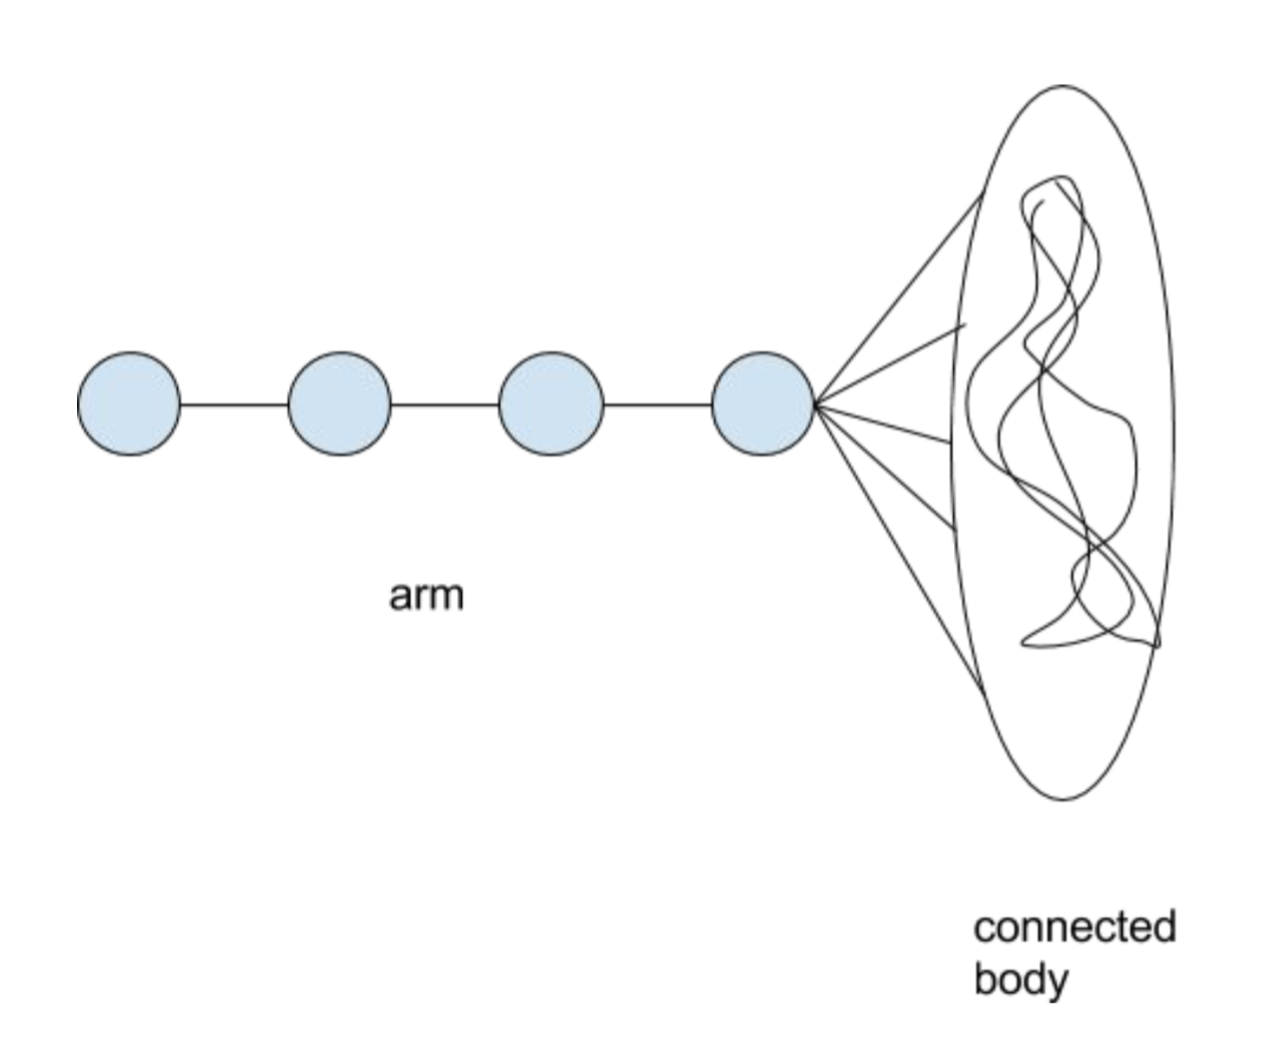
\includegraphics[width=8cm]{graph1}
\end{figure}

%%%%%%%%%%%%%%%%%%%%%%%%%%%%%% Problem 2
\section*{Problem 2}
\subsection*{(a)}
Let H = heads and T = tails.
To get an unbiased bit, we can do the following. We will segment our flips into
rounds of two. That is, if we have the flips HHTTHT, we will consider the results
HH, TT, and HT. Then, if we come across the result HT, we will call that 0. If we
come across the result TH, we will call that 1. We will keep flipping the coin
until we get one of these results. This is unbiased because the probability of
getting HT equals the probability of getting TH, since each flip is independent. \\

\noindent Let $X$ be the number of flips it takes to get one bit. \\
Let $A$ be the event that we get either HT or TH. \\

\noindent Then, to calculate the expected number of flips, we can write the following.

\[ E[X] = 2 P(A) + (2 + E[X]) P(A^c) \]
\[ E[X] = 2 (2p(1 - p)) + (2 + E[X]) (p^2 + (1 - p^2)) \]
\[ E[X] = 4p(1 - p) + (2 + E[X]) (2p^2 - 2p + 1) \]
\[ E[X] = \frac{1}{p - p^2} \]

\noindent The initial equation is explained as follows: when we get either HT or TH, 
then it takes us two flips to get our bit. Else, it takes us two flips plus the 
expected value of flips. The probabilities are fairly straightforward: $P(A)$ 
represents the chance of getting HT or TH, and $P(A^c)$ the chance of getting HH
or TT.

\subsection*{(b)}
Let $K$ be the number of chunks we want to download.  \\
Let $E[K]$ be the expected time to download $k$ chunks. \\
Let $A$ be the event that the randomly selected server has a chunk we have not already
downloaded. \\

\noindent Then we can write the following recurrence relation:

\[ E[K] = P(A)(t_1 + E[K - 1]) + P(A^c)(t_2 + E[K]) \]
\[ E[K] = \frac{K}{n} (t_1 + E[K - 1]) + \frac{n - K}{n} (t_2 + E[K]) \]

\noindent Knowing that $E[0] = 0$, we can solve to get 

\[ E[K] = n t_2 H_K + K(t_1 - t_2) \]

\noindent where $H_K$ is the $K$th harmonic number. The initial equation is explained
as follows. When a server is selected, we know that there are two possibilities.
We can either download a new chunk, which takes time $t_1$ and reduces the remaining
number of chunks by 1; or, we can spend time $t_2$, which leaves us with the same
number of chunks to download. The probabilities for these scenarios are $K / n$
and $(n - K) / n$, respectively.\\

\noindent Then, since we want to download all $n$ chunks, $E[n]$ is the following:

\[ E[n] = n t_2 H_n + n(t_1 - t_2) \]

\subsection*{(c)}
\subsubsection*{(i)}
The probability of getting the first record at time $n$ is the following:

\[ \frac{1}{n - 1} \frac{1}{n} \]

\noindent In words, this represents the following. $\frac{1}{n - 1}$ is the 
probability that the first value is the second biggest and $\frac{1}{n}$ is the 
probability that the current value is the biggest. By doing this, we account
for the fact that a record has not yet occurred (account for the previous $n - 1$
values), while also factoring in the probability that the current variable will 
be the record (account for the current value). Intuitively, this makes
sense. If only 1 value has passed by, the outlook is optimistic that we can beat
the first value. If 1000 values have passed by and none of them have beaten the 
first one, the outlook is a bit more bleak. With this in mind, it becomes easy
to write out the expected value.

\[ E[N] = \sum_{i = 2}^{\infty} i \frac{1}{i - 1} \frac{1}{i} = \infty \]

\subsubsection*{(ii)}
The probability of getting \textit{a} record at time $n$ is simply

\[ \frac{1}{n} \]

\noindent Note that it no longer matters whether or not the record we get is the 
first record, which simplifies the probability expression. Then we can calculate the 
expected number of records that we get within the first $M$ steps. We will call this 
$E[M]$.

\[ E[M] = \sum_{i = 2}^M \frac{1}{i} = \big( \sum_{i = 1}^M \frac{1}{i} \big) - 1 \]

\noindent We do this because the expected number of records we get equals the 
probability of getting a record at step 2 plus the probability of getting a 
record at step 3 plus... etc etc. Then, for large $M$, this becomes

\[ E[M] \approx \ln M - 1 \]

\noindent So to find out what $M$ to choose, we can just solve the following (assuming
$x$ is sufficiently large):

\[ \ln M - 1 = x \]
\[ \ln M = x + 1 \]
\[ M = e^{(x + 1)} \]

%%%%%%%%%%%%%%%%%%%%%%%%%%%%%% Problem 3
\section*{Problem 3}
\subsection*{(a)}
The example for this is fairly simple. First, we have a triangle. Then we
have $n$ vertices, all unconnected. As $n \rightarrow \infty$, $Cl^{avg}$ goes to
$0$. It does this because $Cl_i(G) = 0$ for vertices with degree 0, and as we take
$n \rightarrow \infty$, these dominate the average. $Cl(G)$ is always just $1$, 
because there is $1$ triangle and there are $3$ connected triples. Here is an illustration:

\begin{figure}[h]
    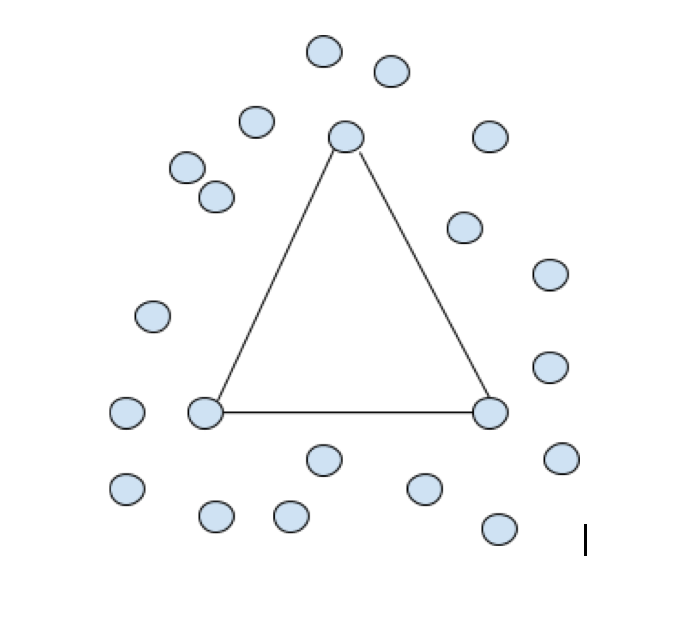
\includegraphics[width=8cm]{graph2}
\end{figure}

%%%%%%%%%%%%%%%%%%%%%%%%%%%%%% Problem 4
\section*{Problem 4}
\subsection*{(a)}
First path (5 nodes): \\
Network congestion (click on \textbf{routers}) $\rightarrow$ Router (computing) 
(click on \textbf{core routers}) $\rightarrow$ Core router 
(click on \textbf{fiber [optic cable]}) $\rightarrow$ Optical fiber (click on
\textbf{electromagnetic interference}) $\rightarrow$ Electromagnetic Interference 
(click on \textbf{capacitor}) $\rightarrow$ Capacitor \\

\noindent Shortest path (4 nodes): \\
Network congestion (click on \textbf{telephone circuits}) $\rightarrow$ Local
loop (click on \textbf{electrical circuit}) $\rightarrow$ Electrical network (click
on \textbf{capacitors}) $\rightarrow$ Capacitors \\

\noindent First path (5 nodes): \\
Paul Erdos (click on \textbf{Mathematics}) $\rightarrow$ Mathematics (click on
\textbf{computer science}) $\rightarrow$ Computer science (click on \textbf{
Distributed computing} $\rightarrow$ Distributed computing (click on 
\textbf{Chandy, Mani}) $\rightarrow$ K. Mani Chandy  \\

\noindent Shortest path (4 nodes): \\
Paul Erdos (click on \textbf{John Selfridge}) $\rightarrow$ 
John Selfridge (click on \textbf{distributed computing}) $\rightarrow$
Distributed computing (click on \textbf{Chandy, Mani}) $\rightarrow$ K. Mani Chandy

\subsection*{(c)}
Note: $>$ indicates continuation of previous line. \\
This problem was done 1/09/16 at around 2:10 pm. My path uses 11 nodes.
\begin{verbatim}
    Star Wars: The Complete Saga (Episodes I-VI) [Blu-ray]
    Leegoal Tri-wing Screwdriver for Nintendo Wii, Gamecube, Gameboy Advance
    45 in 1 Professional Portable Opening Tool Compact Screwdriver Kit Set with 
    > Tweezers & Extension Shaft for Precise Repair or Maintenance Jk6089-A
    SE MH1047L Illuminated Multi-Power LED Head Magnifier
    Pixnor 5-in-1 High-precision Stainless Steel Tweezers Repair Tools Set (Silver)
    Organic Cocoa Butter By Sky Organics: Unrefined, 100% Pure Raw Cocoa Butter 
    > 16oz - Skin Nourishing, Moisturizing & Healing, for Dry Skin, Stretch 
    > Marks - For Skin Care, Hair Care & DIY Recipes 
    Premium Soft Replacement Toothbrush Heads Compatible with Oral B Toothbrush 
    > Handles, 4 Count
    Brio SmartClean Sonic Electric Toothbrush
    Brio Radius Nail Clippers - Toenail Clippers and Fingernail Clippers
    Clorox Disinfecting Wipes Value Pack, Fresh Scent and Citrus Blend, 225 Count
    Colgate Extra Clean Toothbrush, Full Head, Soft, 6 Count
\end{verbatim}

\end{document}
